\documentclass[t, aspectratio=169]{beamer}
\usepackage{amsmath,amsfonts,amsthm,amstext,amssymb, xcolor, tikz, pgf, polynom}

% ----------------------------------------------------------
% Theme Setup

% Use Metropolis Theme
\usetheme[numbering=fraction]{metropolis}
\setbeamertemplate{blocks}[rounded][shadow=false]
\makeatletter
\setlength{\metropolis@titleseparator@linewidth}{1pt}
\makeatother

% Define Colors
\definecolor{chargerblue}{HTML}{002764}
\definecolor{chargerred}{HTML}{e02034}
\definecolor{bggray}{HTML}{d0d3d4}

% Set Colors
\setbeamercolor{title}{fg=chargerblue}
\setbeamercolor{background canvas}{bg=white}
\setbeamercolor{title separator}{fg=chargerred}
\setbeamercolor{structure}{fg=chargerblue}
\setbeamercolor{frametitle}{fg=white, bg=chargerblue}
\setbeamercolor*{normal text}{fg=chargerblue}
\setbeamercolor*{block body}{bg=bggray}
\setbeamercolor*{block title}{bg=chargerblue, fg=white}
% ----------------------------------------------------------

% ----------------------------------------------------------
% Custom Definitions, Commands, Environments, etc.

% Sets of numbers
\def\R{\mathbb{R}} % The reals
\def\N{\mathbb{N}} % The naturals
\def\Z{\mathbb{Z}} % The integers
\def\Q{\mathbb{Q}} % The rationals

% Blank space
\newcommand{\blank}[1]{\underline{\hspace{#1}}} % Blank space

% Fitted inclusion symbols
\newcommand{\fp}[1]{\left({#1}\right)} % Fitted parentheses around content
\newcommand{\fb}[1]{\left[{#1}\right]} % Fitted brackets
\newcommand{\set}[1]{\left\{{#1}\right\}} % Fitted braces (useful for sets)
\newcommand{\av}[1]{\left|{#1}\right|} % Fitted absolute value bars



% Coordinate Plane (Four-Quadrant)
\def\coordplane {
	\begin{tikzpicture}		\draw[step=0.25cm,black,very thin,opacity=0.25] (-2.5cm, -2.5cm) grid (2.5cm, 2.5cm);
	\draw[<->,thick,black] (-2.5cm, 0) -- (2.5cm, 0) node[anchor=north west,pos=0.94,font=\scriptsize]{$x$};
	\draw[<->,thick,black] (0,-2.5cm) -- (0, 2.5cm) node[anchor=south east,font=\scriptsize,pos=0.94]{$y$};
	\end{tikzpicture}
}

% Coordinate Plane (One-Quadrant)
\def\onequad {
	\begin{tikzpicture}
	\draw[step=0.25cm, black, very thin, opacity=0.25] (0,0) grid (7.5cm,5cm);
	\draw[->, thick, black] (0,0) -- (7.5cm, 0) node[anchor=north west,font=\scriptsize,pos=0.94]{$x$};
	\draw[->, black, thick] (0,0) -- (0,5cm) node[anchor=south east,font=\scriptsize,pos=0.94]{$y$};
	\end{tikzpicture}
}
% ----------------------------------------------------------

% ----------------------------------------------------------
% Presentation Information 
\title[4.2]{Graphing Rational Functions}
\subtitle{Section 4.2}
\author{Jacob Ayers}
\institute{Lesson \#16}
\date{MAT 130}
% ----------------------------------------------------------

\begin{document}
	
	% Slide 1 (Title Slide)
	\begin{frame}
		\titlepage
	\end{frame}
	
	% Slide 2 (Objectives)
	\begin{frame}{Objectives}
		\begin{itemize}
			\item Sketch graphs of rational functions
			\item Sketch graphs of rational functions that have slant asymptotes
		\end{itemize}
	\end{frame}
	
	\begin{frame}{Graphing Rational Functions}
		\begin{block}{Guidelines for Graphing Rational Functions}
			\begin{enumerate}[1)]
				\item Simplify the function if you can. Be sure to list any restrictions on the domain that aren't implied by the simplified function. \pause
				\item Find and plot the $y$-intercept by evaluating $f(0)$. \pause
				\item Find and plot the $x$-intercept(s) by setting the numerator to $0$ and solving. \pause
				\item Find and sketch any vertical asymptotes by setting the denominator to $0$ and solving. \pause
				\item Find and sketch any horizontal asymptotes. \pause
				\item Plot additional points as necessary. \pause
				\item Use smooth curves to complete the graph.
			\end{enumerate}
		\end{block}
	\end{frame}

	\begin{frame}{Graphing Rational Functions}
		Sketch the graph of $\dfrac{1}{x+3}$ and state its domain. \pause
		
		1) The function can't be simplified. Its domain is $x \neq -3$. \pause
		
		2) $f(0) = \dfrac{1}{0+3} = \dfrac13$ so the $y$-intercept is at $\fp{0,\dfrac13}$. \pause
		
		3) The numerator will never be zero. There are no $x$-intercepts. \pause
		
		4) The denominator will be zero when $x = -3$. There is a vertical asymptote at $x = -3$. \pause
		
		5) The degree of the numerator is less than the degree of the denominator. There is a horizontal asymptote at $y = 0$.
	\end{frame}

	\begin{frame}{Graphing Rational Functions}
		6) Based on the current state of our graph, we need several points: \pause
		
		\begin{tabular}{c|ccccccc}
			$x$ & $-1$ & $-2$ & $-2.5$ & $-3.5$ & $-4$ & $-5$ & $-6$ \\ \hline
			$f(x)$ & $\dfrac12$ & $1$ & $2$ & $-2$ & $-1$ & $-\dfrac12$ & $-\dfrac13$
		\end{tabular} \pause
	
		7) 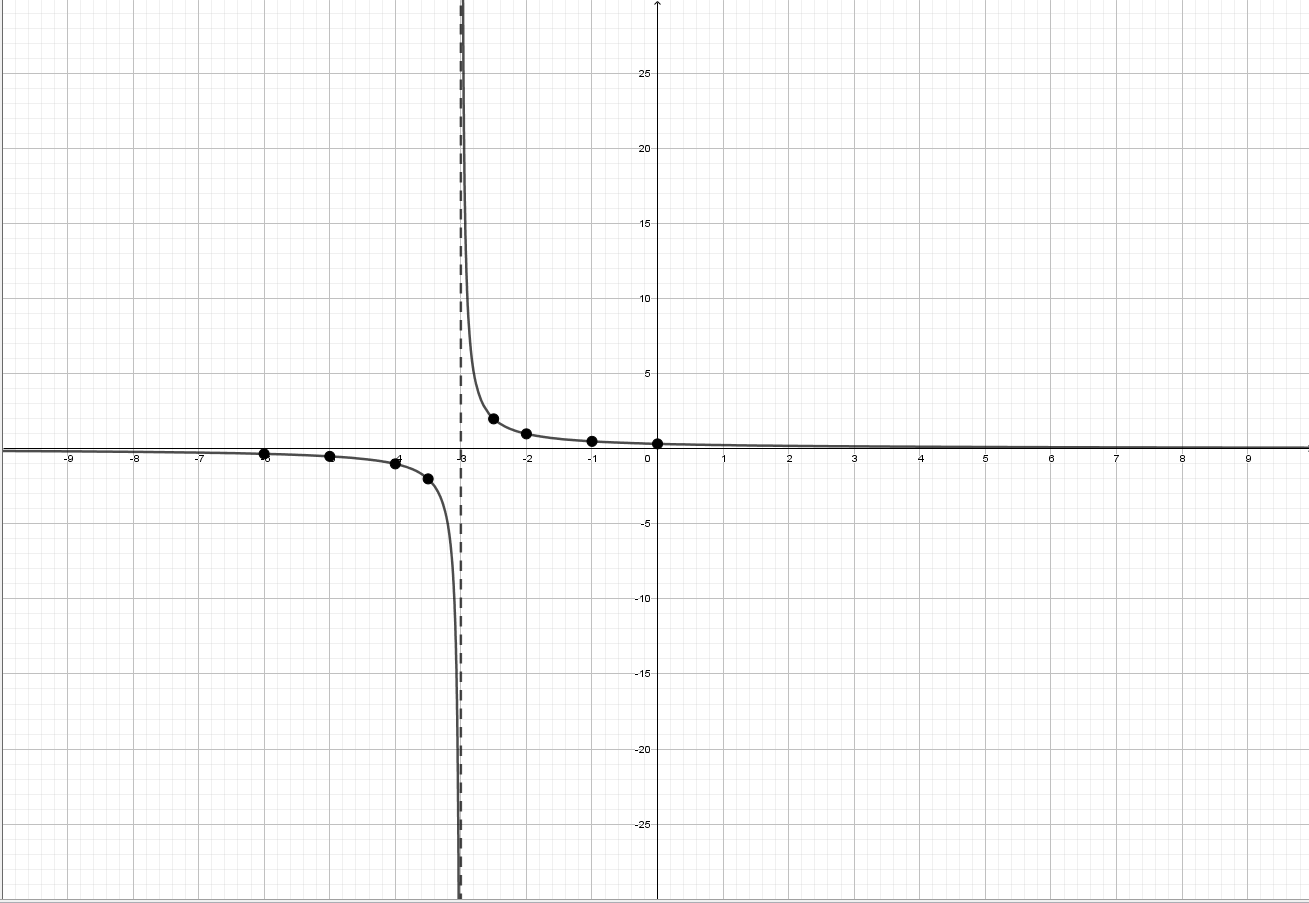
\includegraphics[width=2.5in]{Rat1.png}
	\end{frame}

	\begin{frame}{Graphing Rational Functions}
		Sketch the graph of $g(x) = \dfrac{3 + 2x}{1 + x}$ and state its domain. \pause
		
		1) The function can't be simplified, but we should write the numerator and denominator in standard form; $g(x) = \dfrac{2x + 3}{x+1}$. The domain is $x \neq -1$. \pause
		
		2) $f(0) = 3$ so the $y$-intercept is $(0,3)$. \pause
		
		3) The numerator is $0$ when $x = -\dfrac32$ so there is an $x$-intercept at $\fp{-\dfrac32, 0}$. \pause
		
		4) The denominator is $0$ when $x = -1$ so there is a vertical asymptote at $x = -1$.
	\end{frame}

	\begin{frame}{Graphing Rational Functions}
		5) The degrees of the numerator and the denominator are the same, so there is a horizontal asymptote at $y = \frac{2}{1} = 2$. \pause
		
		6) We could use some more points on each side of the asymptote. \pause
		
		\begin{tabular}{c|ccccccc}
			$x$ & $-2$ & $-3$ & $-4$ & $-0.5$ & $1$ & $2$ \\ \hline
			$f(x)$ & $1$ & $1.5$ & $1.67$ & $4$ & $2.5$ & $2.33$
		\end{tabular}
	\end{frame}

	\begin{frame}{Graphing Rational Functions}
		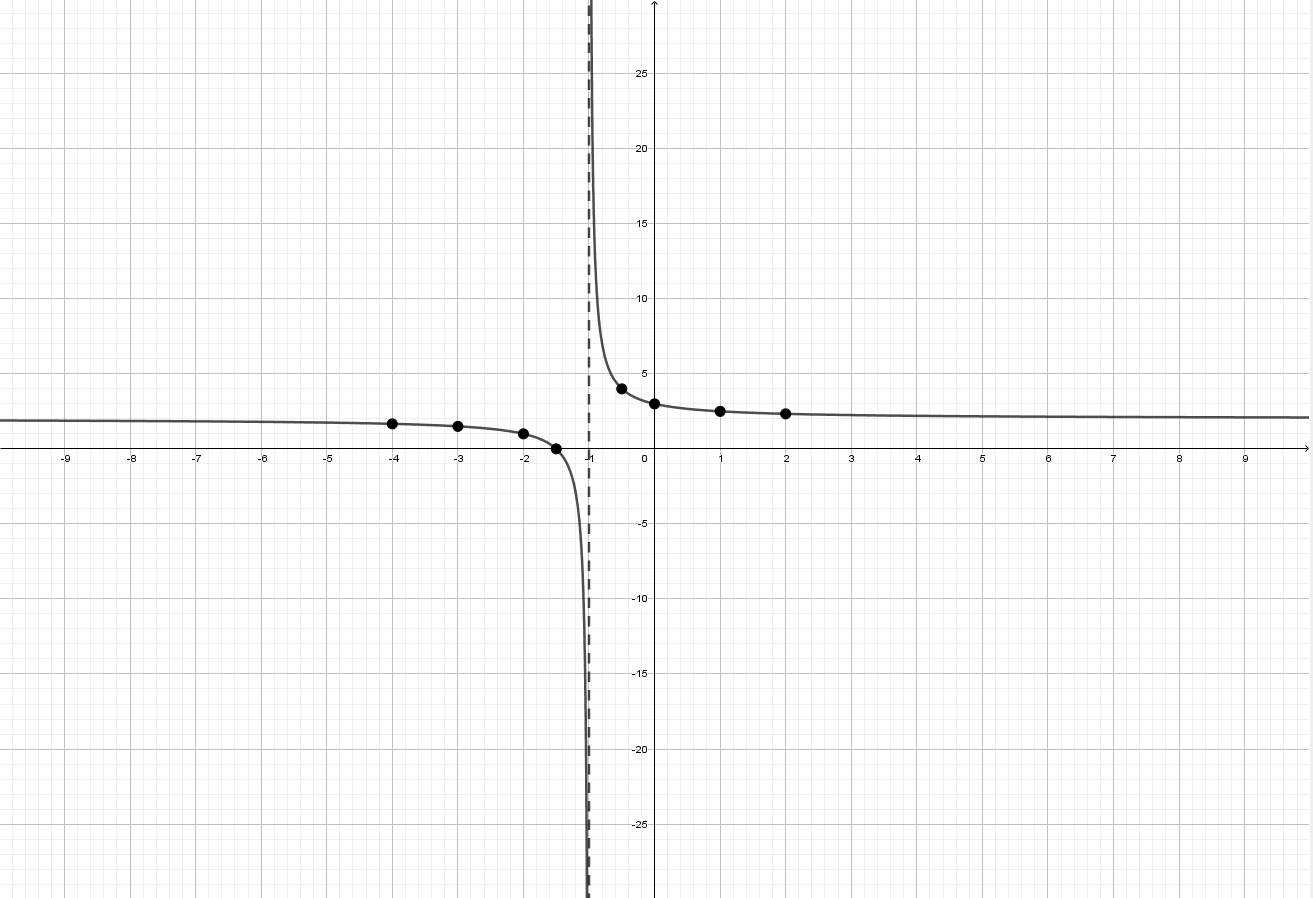
\includegraphics[width=4in]{Rat2.png}
	\end{frame}

	\begin{frame}{Graphing Rational Functions}
		Sketch the graph of $f(x) = \dfrac{x^2 - 4}{x^2 - x - 6}$ and state its domain. \pause
		
		1) We can simplify this function: $f(x) = \dfrac{(x+2)(x-2)}{(x-3)(x+2)} = \dfrac{x-2}{x-3}, x\neq -2$ \\
		Its domain is $x \neq -2, 3$. \pause
		
		2) $f(0) = \dfrac23$ so the $y$-intercept is $\fp{0,\dfrac23}$. \pause
		
		3) The numerator will be zero when $x = 2$, so there is an $x$-intercept at $(2,0)$. \pause
		
		4) The denominator will be zero when $x = 3$ so there is a vertical asymptote at $x = 3$.
	\end{frame}

	\begin{frame}{Graphing Rational Functions}
		5) The degree of the numerator and denominator are the same, so there is a horizontal asymptote at $y = \frac{1}{1} = 1$. \pause
		
		6) We could use some points on each side of the vertical asymptote. \pause
		
		\begin{tabular}{c|ccccc}
			$x$ & $1$ & $2.5$ & $3.5$ & $4$ & $5$ \\ \hline
			$f(x)$ & $0.5$ & $-1$ & $3$ & $2$ & $1.5$
		\end{tabular}
	\end{frame}

	\begin{frame}{Graphing Rational Functions}
		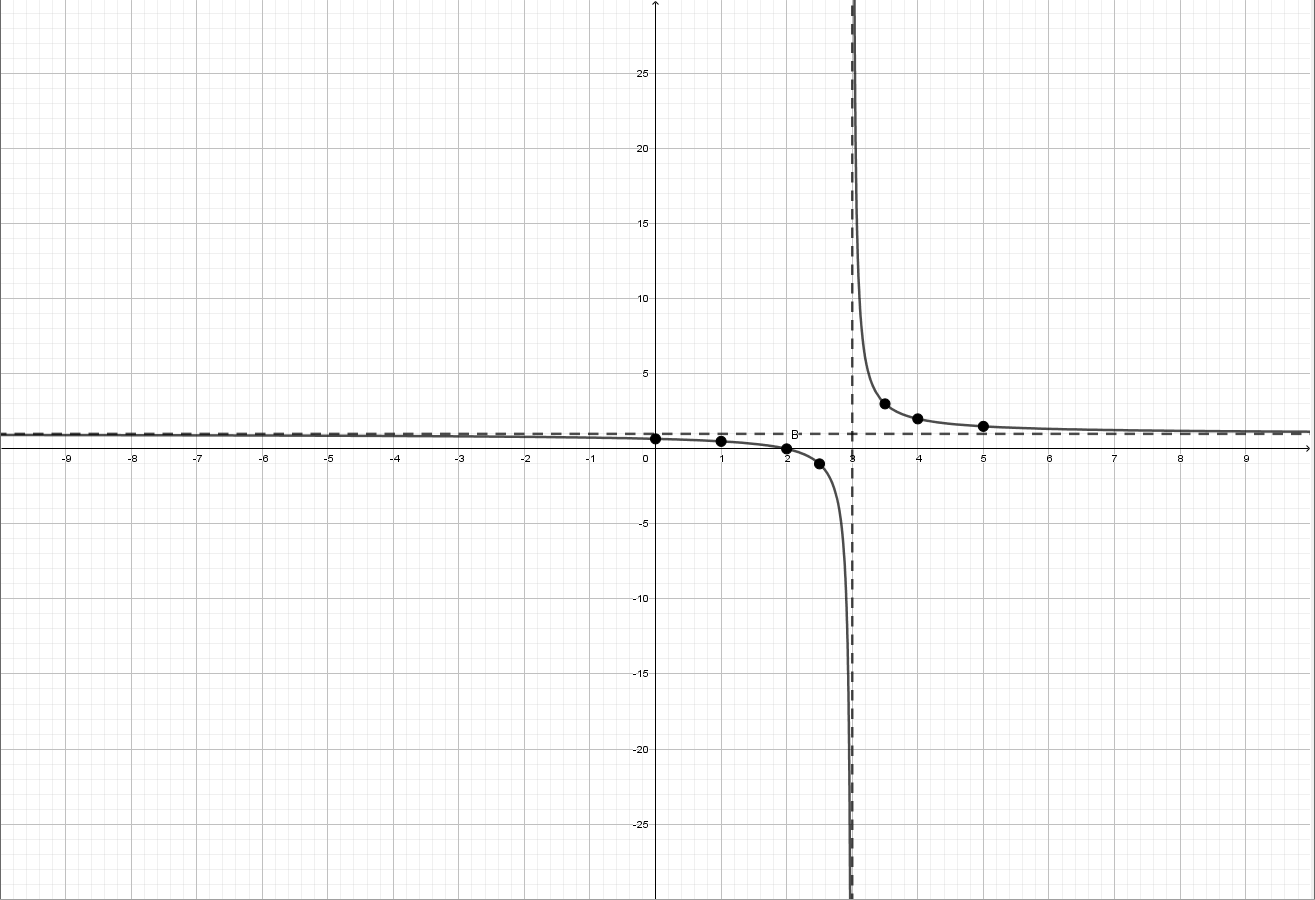
\includegraphics[width=4in]{Rat3.png}
	\end{frame}

	\begin{frame}{Slant Asymptotes}
		When the degree of the denominator is at least $1$, and the degree of the numerator is exactly one more than the numerator, the graph will have a \textit{slant asymptote} rather than a horizontal asymptote. \pause
		
		To find the equation of the slant asymptote, we divide the numerator by the denominator (using long division or synthetic division), and the non-remainder portion is the equation for the slant asymptote.
	\end{frame}

	\begin{frame}{Slant Asymptotes}
		Find the equation for the slant asymptote for the function $f(x) = \dfrac{x^2 + 5x + 6}{x-8}$. \pause
		
		Since the divisor is of the form $x - k$, we can use synthetic division. \pause
		
		\polyhornerscheme[x=8]{x^2 + 5x + 6}
		
		Based on this result, we conclude that the slant intercept is $y = x + 13$
	\end{frame}

	\begin{frame}{Graphing Functions with Slant Asymptotes}
		Sketch the graph of $f(x) = \dfrac{3x^2 + 1}{x}$ and state its domain. \pause
		
		1) This function can't be simplified. Its domain is $x \neq 0$. \pause
		
		2) $f$ is undefined at $0$; there is no $y$-intercept. \pause
		
		3) The numerator will never be $0$; there is no $x$-intercept. \pause
		
		4) The denominator is $0$ when $x = 0$; there is a vertical asymptote at $x = 0$.
	\end{frame}

	\begin{frame}{Graphing Functions with Slant Asymptotes}
		5) The degree of the numerator is \textit{exactly one more} than the degree of the denominator. There is no horizontal asymptote, but there will be a slant asymptote and we can find it using synthetic division (with $k = 0$): \pause
		
		\polyhornerscheme[x=0]{3x^2 + 1} \pause
		
		The equation of the slant asymptote is $y = 3x$.
	\end{frame}

	\begin{frame}{Graphing Functions with Slant Asymptotes}
		6) We have no points. We could use points on each side of the vertical asymptote. \pause
		
		\begin{tabular}{c|cccccccc}
			$x$ & $0.5$ & $1$ & $2$ & $3$ & $-0.5$ & $-1$ & $-2$ & $-3$ \\ \hline
			$f(x)$ & $3.5$ & $4$ & $6.5$ & $9.33$ & $-3.5$ & $-4$ & $-6.5$ & $-9.33$
		\end{tabular} \pause
	
		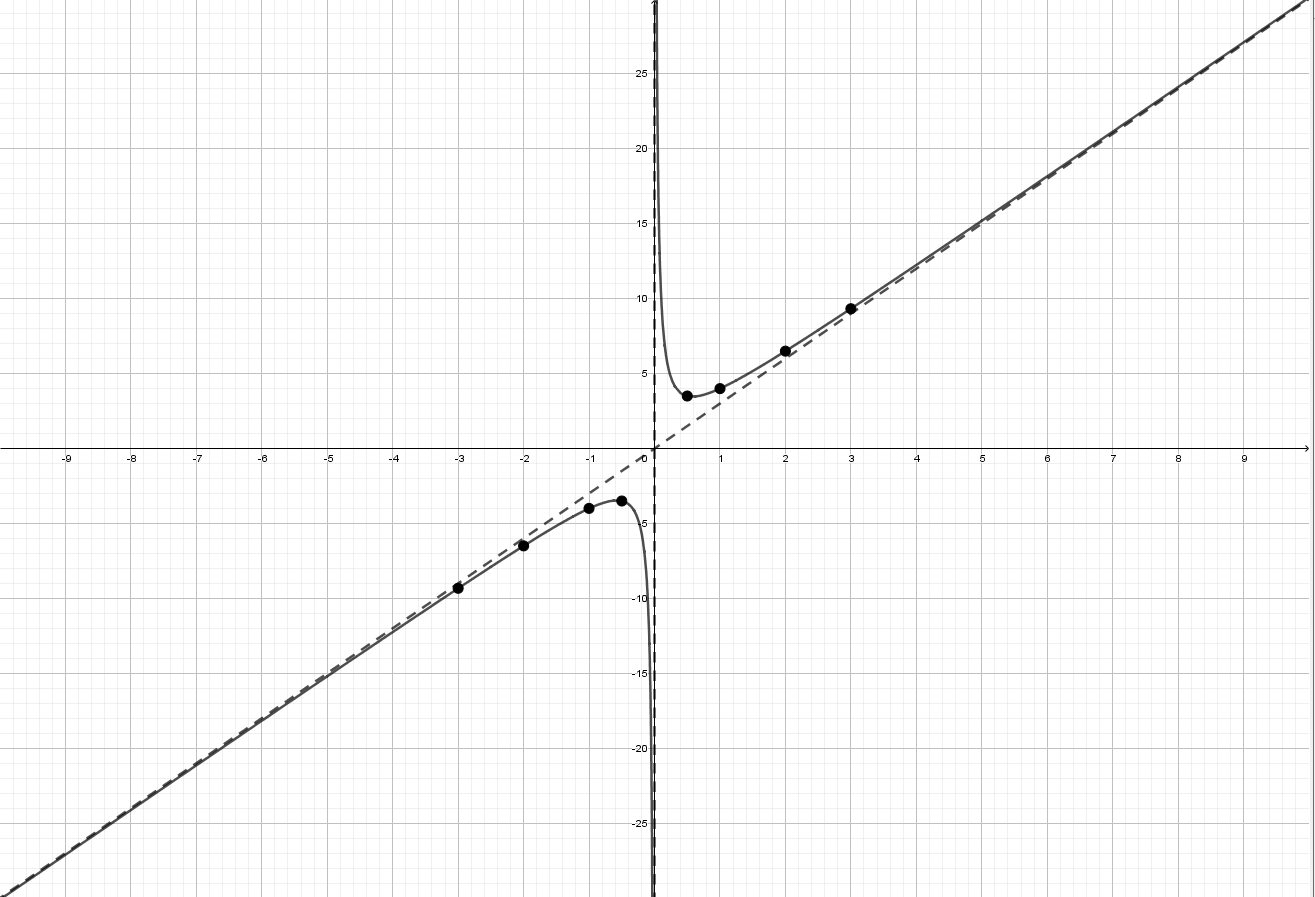
\includegraphics[width=3in]{Rat4.png}
	\end{frame}

	\begin{frame}{Next Steps}
		\begin{itemize}
			\item Ask questions in Lesson 16 Forum, if you have any
			\item Read 5.1
			\item Watch Video Lesson \#17
			\item Complete Assignment \#8 
		\end{itemize}
	
	\vfill
	
	Thanks for watching!
	\end{frame}
\end{document}